\documentclass[10pt]{article}

% ---------- Page geometry (kept tight: 10-page hard cap) ----------
\usepackage[margin=0.75in,top=0.7in,bottom=0.75in]{geometry}
\usepackage{fontspec}
\usepackage{polyglossia}
\setmainlanguage{english}
\setotherlanguage{hindi}
\newfontfamily\devanagarifont{Noto Sans Devanagari}
\newcommand{\dn}[1]{{\devanagarifont #1}}

\usepackage{graphicx}
\usepackage{booktabs}
\usepackage{array}
\usepackage{caption}
\usepackage[table]{xcolor}
\usepackage{titlesec}
\usepackage{enumitem}
\usepackage[colorlinks=true,linkcolor=blue,urlcolor=blue,citecolor=blue]{hyperref}
\usepackage{multicol}
\usepackage{amsmath}

% Compact section spacing to fit 10 pages
\titlespacing*{\section}{0pt}{6pt}{3pt}
\titlespacing*{\subsection}{0pt}{4pt}{2pt}
\setlength{\parskip}{2pt}
\setlength{\parindent}{0pt}
\captionsetup{font=small,skip=2pt}
\setlist{noitemsep, topsep=2pt, leftmargin=1.2em}

\renewcommand{\arraystretch}{1.0}
\newcolumntype{L}[1]{>{\raggedright\arraybackslash}p{#1}}

\titleformat{\section}{\normalfont\large\bfseries}{\thesection}{0.6em}{}
\titleformat{\subsection}{\normalfont\bfseries}{\thesubsection}{0.6em}{}

\title{\vspace{-1.5em}\textbf{Monolingual Transformer LMs in Hindi and Nepali}\\
\large Consolidated Final Report --- Phases 1--3}
\author{Language Models and Agents, Monsoon 2026 --- Individual Project}
\date{\small Model H = Hindi (higher-resource) \quad Model L = Nepali (lower-resource) \quad Branch: \texttt{phase-3}}

\begin{document}
\maketitle
\vspace{-2.2em}

\begin{center}\small
Two independently trained, from-scratch, decoder-only Transformer LMs ($\sim$25M params each), one per language.
No pretrained weights, tokenizers, or shared vocabulary between them.
Every number below is generated from metric JSON the pipeline scripts produced.
Full per-phase detail: \texttt{report/phase1\_report.md}, \texttt{phase2\_report.md}, \texttt{phase3\_report.md}.
\end{center}
\vspace{-0.3em}

%=====================================================================
\section{Phase 1 --- Data Collection and Tokenizer Construction}
%=====================================================================

\textbf{Language choice.} Model H = Hindi: best-represented Indian language in IndicCorpV2 (3 shards) with a usable Wikipedia dump, giving headroom to spend the manual lane on source diversity. Model L = Nepali: IndicCorpV2 ships it as a single file, no usable Wikisource wiki exists, forcing a news-only manual lane --- a direct, measurable resource gap. Both share Devanagari script, so H-vs-L differences are attributable to resource level and language, not script.

\textbf{Pipeline.} Identical 12-stage streaming pipeline for both languages, zero shared code/data/tokenizer beyond generic utilities in \texttt{shared/}: download $\to$ normalize $\to$ script-filter $\to$ quality-filter $\to$ dedup (exact + MinHash/LSH) $\to$ corpus stats $\to$ split (90/5/5, frozen val/test) $\to$ decontaminate train against frozen val/test $\to$ concatenate $\to$ train tokenizer $\to$ evaluate tokenizer $\to$ tokenize.

\textbf{Two design choices, and why they were made this way.}
\emph{Split before decontamination.} Val/test are written once, frozen, and never touched again \emph{before} the tokenizer is trained and before decontamination. The alternative --- decontaminate first, then split --- would let decontamination's own similarity threshold implicitly influence which lines end up in val/test, making the held-out set a function of a design choice rather than a genuinely independent sample. Freezing first means held-out perplexity in Phase 2 is measured on text the pipeline never adapted around, and the tokenizer never sees a single held-out line either.
\emph{Deduplication has source precedence, not arbitrary tie-breaking.} When identical/near-identical text exists in both a manual source and IndicCorp, the manual copy is kept (Hindi: Wikipedia $>$ News $>$ IndicCorp; Nepali: Onlinekhabar $>$ Khabarhub $>$ IndicCorp). This was a deliberate choice, not a default: the $\geq$20\% manual-fraction requirement would be trivially threatened if a dedup pass discarded manual copies in favor of IndicCorp duplicates, so precedence protects the harder-to-satisfy sub-target at the easier one's expense.

\textbf{Script-filter and dedup threshold choices.} Devanagari-ratio gates were set at 0.60 (Hindi) vs.\ 0.70 (Nepali) --- lower for Hindi specifically because Hindi news is measurably more code-mixed with English (confirmed later by the 6.00\% Latin-content statistic in \S\ref{sec:corpus-health} below, a diagnosis made from the aggregate statistic, not from reading borderline lines). The near-duplicate MinHash/LSH threshold (Jaccard 0.4, 32 permutations, 3-word shingles) was chosen deliberately aggressive --- it removes text a human might judge distinct --- because the cost of an under-aggressive threshold (train/test leakage in the frozen val/test sets) is worse than the cost of over-pruning train candidates, especially since both corpora exceeded their token targets by 26--28\% with room to spare. Decontamination reuses the same mechanism but at a \emph{looser} setting (16 permutations, 5-word shingles) than dedup's 32/3-word setting --- recall matters more than precision when a miss means genuine train/test leakage, so decontamination is tuned to over-remove rather than under-remove.

\begin{table}[h]
\centering\small
\begin{tabular}{lrr}
\toprule
& \textbf{Model H (Hindi)} & \textbf{Model L (Nepali)} \\
\midrule
Final train tokens (content) & 632,352,544 & 637,535,988 \\
Manual-lane tokens (\% of train) & 114,417,599 (18.1\%) & 116,842,022 (18.3\%) \\
Manual sources & Wikipedia + 3 news outlets & 2 news outlets (WordPress API) \\
Unique whitespace words & 3,956,492 & 6,800,829 \\
Vocabulary size (selected) & 12,000 & 12,000 \\
Tokenizer fertility (tok/word) & \textbf{1.3042} & \textbf{1.4394} \\
UNK rate (all vocab sizes) & 0.0000 & 0.0000 \\
\bottomrule
\end{tabular}
\caption{Phase 1 headline numbers. Both languages exceed the $\sim$500M-token and $\geq$20\% manual-fraction targets; no shortfall justification is needed for either.}
\end{table}

\textbf{Vocabulary size (12,000, both languages).} Fertility falls monotonically with vocab size in both languages, so no size is optimal on compression alone; 12K is where the \emph{marginal} fertility gain per 2,000 added rows starts shrinking, for both languages simultaneously, and keeping the same size for H and L keeps Phase 2 perplexity comparisons uncontaminated by a vocabulary-size confound.

\textbf{Nepali's higher fertility is morphology, not corpus quality.} Nepali is agglutinative (postpositions fuse onto stems, e.g. \dn{नेपालको} = \dn{नेपाल} + \dn{को}), which is why it has \emph{more} unique surface forms (6.80M vs.\ 3.96M) despite being the lower-resource language, and why BPE needs 10.4\% more tokens per word to cover it. This single fact is the root cause traced through Phases 2--3 below.

\textbf{Corpus composition and health.}\label{sec:corpus-health} Devanagari purity is $\geq$90\% in every source for both languages, confirming the script filter works. Hindi's news lane carries 6.00\% Latin content --- the highest of any source, and real: Hindi news outlets routinely embed English proper nouns and brand names. Nepali's news sources are purer ($\geq$98.8\% Devanagari), reflecting a less code-mixed newsroom register. Document length is the more consequential composition fact: news articles average 1,499--2,494 characters while IndicCorp lines are sentence/paragraph fragments (218--286 characters) --- a manual document is worth roughly 7--10 IndicCorp documents in token terms, which is why the manual lane reaches $\sim$18\% of tokens from only $\sim$3--8\% of documents. Every manual-fraction number in this report is therefore \textbf{token-weighted}, not document-count-weighted, since the latter would badly understate the manual lane's real contribution.

\begin{figure}[h]
\centering
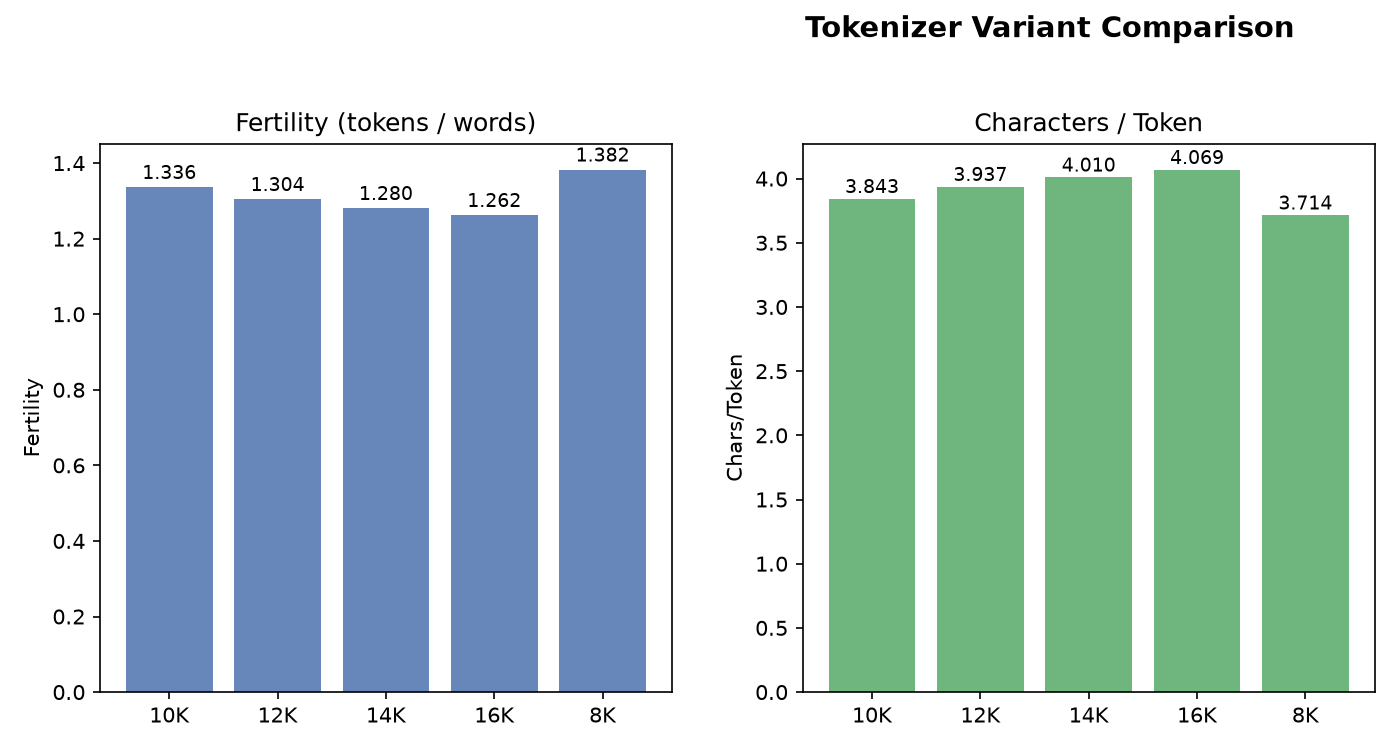
\includegraphics[width=0.48\textwidth]{../figures/hindi/tokenizer_comparison_hin.png}
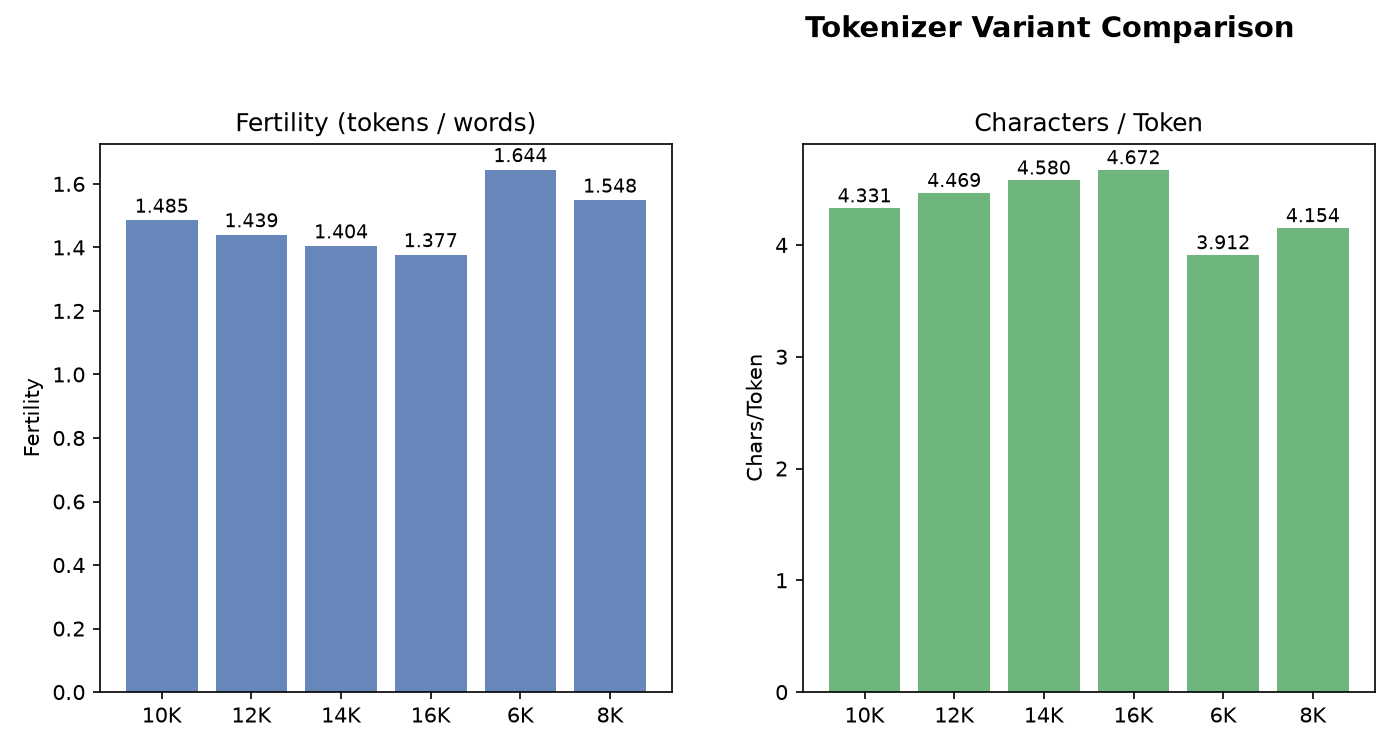
\includegraphics[width=0.48\textwidth]{../figures/nepali/tokenizer_comparison_nep.png}
\caption{Fertility and chars/token across candidate vocabulary sizes, held-out validation. Hindi (left) is consistently more compressible than Nepali (right) at every matched vocabulary size.}
\end{figure}

\begin{table}[h]
\centering\small
\begin{tabular}{lrrl}
\toprule
\textbf{Requirement} & \textbf{Hindi} & \textbf{Nepali} & \textbf{Status} \\
\midrule
$\sim$500M training tokens & 632,352,544 & 637,535,988 & \textbf{PASS} --- both exceed by 26--28\% \\
IndicCorp sub-target 400M & 517,934,945 & 520,693,966 & \textbf{PASS} \\
Manual sub-target $\geq$100M & 114,417,599 (+14.4\%) & 116,842,022 (+16.8\%) & \textbf{PASS} \\
Tokenizer trained from scratch & yes & yes & \textbf{PASS} \\
No shared tokenizer/vocab/data & yes & yes & \textbf{PASS} \\
Train decontaminated vs.\ val/test & yes & yes & \textbf{PASS} \\
\bottomrule
\end{tabular}
\caption{Phase 1 requirement compliance, both languages.}
\end{table}

%=====================================================================
\section{Phase 2 --- Model, Pretraining, and Evaluation}
%=====================================================================

{\sloppy\textbf{Architecture.} Decoder-only Transformer built \emph{only} from \texttt{nn.Linear}, \texttt{nn.Embedding}, \texttt{nn.LayerNorm}, \texttt{nn.Dropout} --- no \texttt{nn.Transformer*}, no \texttt{nn.MultiheadAttention}, no HuggingFace, and deliberately no fused \texttt{scaled\_dot\_product\_attention}: a pre-built fused kernel would hide exactly the softmax/mask mechanics this phase is meant to demonstrate understanding of.\par} 6 layers, 8 heads, $d_{\text{model}}=512$, $d_{ff}=2048$, block size 512, learned absolute positions, pre-norm, GELU, weight tying. \textbf{25,321,472} parameters, identical for both languages so that any H-vs-L difference in results is attributable to data/language, not architecture. Causal masking verified bit-exact (max $|\Delta|=0$ at all positions $\le t$ under a future-token perturbation, both models; a second independent check confirms every attention row places zero weight on future keys).

\textbf{Why these specific choices, not others.}
\emph{Depth $\times$ width (6 layers $\times$ 512) over alternatives at the same $\sim$25M budget} --- e.g.\ 12 layers $\times$ 384 ($d_{ff}$ scaled accordingly, also $\approx$26.1M params). Weight tying (reusing the token-embedding matrix as the output head, since both map between the same vocabulary/representation space) frees 6.14M parameters --- 19.5\% of the untied 31.47M total --- and that freed budget was spent on width rather than depth: wider matmuls (head\_dim $=512/8=64$) use the GPU more efficiently per parameter than a deeper, narrower stack, and at $\sim$650M training tokens for a 25M-parameter model, data volume rather than representational depth is the binding constraint (Chinchilla-optimal for 25M params is $\sim$500M tokens; both corpora exceed that).
\emph{Pre-norm over post-norm.} $x + \text{Sublayer}(\text{LN}(x))$ keeps the residual stream an unbroken identity path, so gradients reach layer 0 without passing through a LayerNorm Jacobian at every layer; post-norm compounds that factor multiplicatively with depth and needs careful warmup to avoid early divergence. This mattered concretely here: each pretraining run had to survive a session-limited cloud GPU environment, so stable convergence from step 0 (no warmup-divergence risk) was worth more than post-norm's marginally different final-loss properties at this scale.
\emph{$1/\sqrt{d_k}$ attention scaling.} For unit-variance $Q,K$, the dot product over $d_k=64$ terms has variance 64 (std 8); an unscaled softmax over logits that large saturates and its gradient vanishes. Dividing by $\sqrt{d_k}$ restores unit variance and keeps softmax in its responsive range --- without this, attention would stop learning early in training regardless of other hyperparameters.
\emph{Learned absolute positions over sinusoidal/RoPE.} Chosen for implementation transparency (a directly inspectable $512\times512$ embedding table) at the cost of a hard 512-token context ceiling --- acceptable here since reasoning-task prompts (Phase 3) and generation-eval prefixes (Phase 2) are both well under that length.

\textbf{Pretraining setup and why.} AdamW (betas 0.9/0.95, weight decay 0.1 applied only to 2-D weight matrices --- LayerNorm gains and biases are excluded since decaying them has no regularizing benefit and can destabilize normalization). Peak LR $6\times10^{-4}$ with 2\% linear warmup then cosine decay to $6\times10^{-5}$: warmup avoids a large-batch cold-start instability at the highest LR, and cosine decay (rather than a step schedule) gives a smooth, hyperparameter-light annealing appropriate for a single-epoch budget where there is no second cycle to tune against. Effective batch $32\times512\times3\text{ accum}=49{,}152$ tokens/step, gradient clipping 1.0, AMP fp16 with a \texttt{GradScaler} --- fp16 (not bf16) was the available precision on the target 2$\times$T4 hardware, so the scaler is load-bearing rather than optional. \textbf{One epoch is the deliberate budget, not a compute shortfall}: both corpora (648M/660M tokens) already exceed the $\sim$500M Chinchilla-optimal point for 25M parameters, so a second epoch would mostly buy memorization risk rather than genuine capability. Every checkpoint carries model weights, optimizer state, scheduler state, AMP scaler state, step count, tokens-seen, and the full config; checkpoint/resume was verified \textbf{bit-exact} before the real runs (40 uninterrupted steps vs.\ 20 steps + kill + resume $\to$ 0 tensor-element difference) specifically because Colab/Kaggle sessions terminate without warning, and an unverified resume path would risk silently corrupting a multi-hour run discovered only after the fact.

\begin{table}[h]
\centering\small
\begin{tabular}{lrr}
\toprule
\textbf{Metric} & \textbf{Model H (Hindi)} & \textbf{Model L (Nepali)} \\
\midrule
Training tokens (1 epoch) & 648,012,574 & 659,499,440 \\
Optimizer steps & 13,183 & 13,417 \\
Training wall-clock (h, 2$\times$T4) & 2.56 & 2.62 \\
\textbf{Validation cross-entropy (nats/token)} & 3.2662 & 3.7262 \\
\textbf{Validation perplexity} & 26.21 & 41.52 \\
\textbf{Validation bits-per-byte (BPB)} & 0.4797 & 0.4635 \\
Test perplexity / BPB & 26.19 / 0.4791 & 41.46 / 0.4632 \\
Mean attention entropy (nats) & 1.3109 & 1.2671 \\
Mean attention distance (tokens) & 3.98 & 3.84 \\
\bottomrule
\end{tabular}
\caption{Phase 2 headline results, validation and test.}
\end{table}

\textbf{The central finding: the H/L gap reverses sign depending on the unit.} In token space, Model L looks 58.4\% worse (PPL 41.52 vs.\ 26.21). In byte space (BPB, tokenizer-independent), Model L is 3.4\% \emph{better} (0.4635 vs.\ 0.4797) --- confirmed on the held-out test split (+58.3\% / $-$3.3\%), so it is not a validation-set artifact. \textbf{Perplexity is denominated in each model's own tokenizer}: because Nepali's fertility is 10.4\% higher, Model L sees less linguistic content per fixed-size training batch, making its per-token prediction problem intrinsically harder --- a tokenizer/morphology artifact, not a resource-level modelling failure. This is exactly the reversal the BPB metric exists to catch, and it recurs, restated, in Phase 3's reasoning results (\S\ref{sec:p3}).

\begin{figure}[h]
\centering
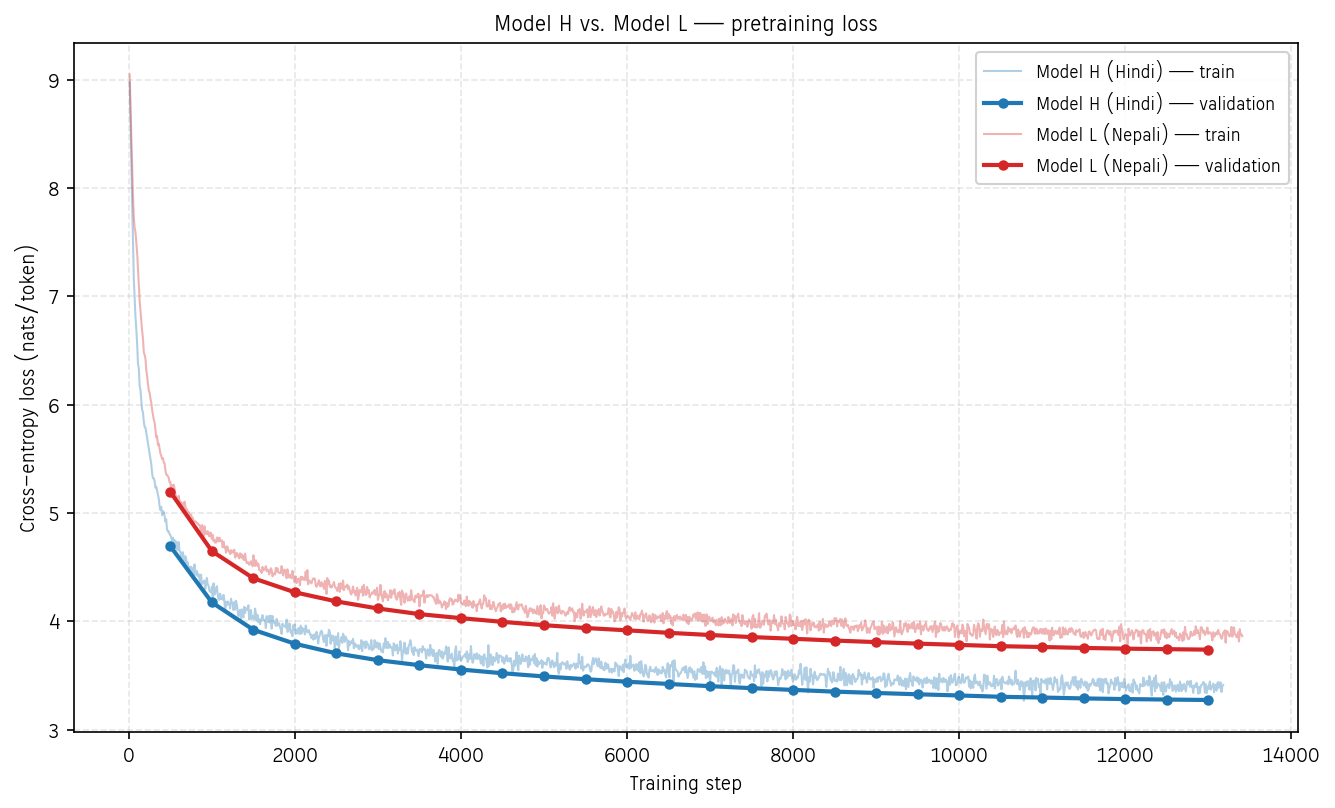
\includegraphics[width=0.48\textwidth]{../figures/comparison/loss_curves_both.png}
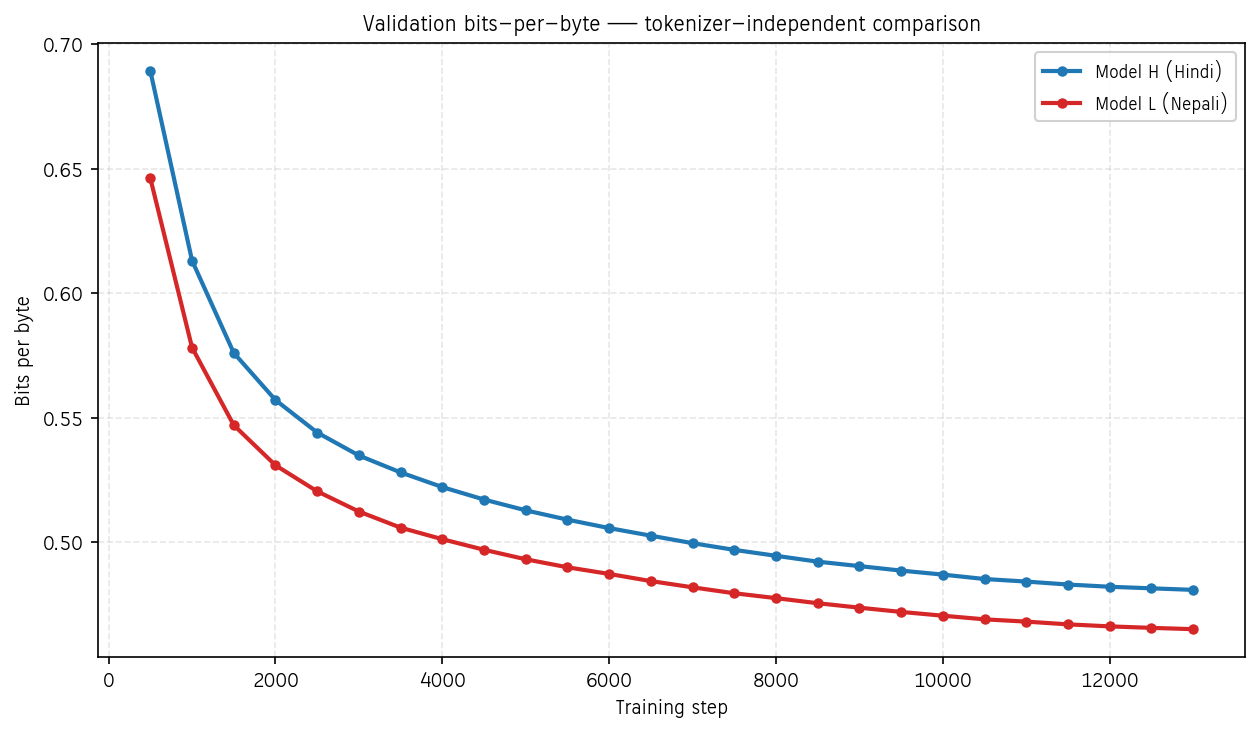
\includegraphics[width=0.48\textwidth]{../figures/comparison/bpb_curves_both.png}
\caption{Left: training loss, both models, smooth convergence with no divergence. Right: validation BPB over training --- the Model L $<$ Model H ordering holds from step 500 onward, not just at the final checkpoint.}
\end{figure}

\textbf{Generation quality: why four different metrics, not one.} 500 held-out prefixes (32-token), greedy + temperatures 0.5/1.0/1.5, scored against the true continuation using each language's \emph{own} SentencePiece pieces rather than whitespace tokens (whitespace tokenization would score two near-identical continuations at zero, given Nepali's 6.80M vs.\ Hindi's 3.96M unique whitespace words from Phase 1). \textbf{BLEU-4 is near-uninformative here, and that is the correct diagnosis rather than a failure}: a 25M model continuing open-ended text against a \emph{single} reference has no realistic path to 4-gram overlap (scores $<$1, occasionally exactly 0 at T=1.5 for Hindi) --- BLEU was designed for translation, where the reference genuinely constrains the output, and open-ended continuation has no such constraint. \textbf{chrF is the most informative of the three overlap metrics}, since character n-grams credit a generation that gets the stem right but inflects differently --- exactly the dominant case in Devanagari morphology --- and it is the only one that rises monotonically with temperature (H: 7.16$\to$18.44; L: 6.71$\to$20.84). ROUGE-L sits between the two, peaking at T=1.0 since LCS rewards in-order overlap without demanding contiguity. \textbf{The diversity diagnostics matter more than the overlap metrics}: greedy decoding shows severe repetition (rate 0.70 H / 0.76 L) that BLEU/chrF barely penalize, since a model that loops one phrase forever can still score respectably on overlap. Distinct-2 rises from $\sim$0.19 to $\sim$0.95 for both languages across the temperature sweep as repetition collapses to near zero --- no single metric captures generation quality alone, which is the reason all four are reported together rather than picking one.

Qualitative spot-check (greedy, Hindi): prompt ``\dn{...ग्रामीण अर्थव्यवस्था पूरी तरह चर}'' $\to$ generated ``\dn{विकास के लिए सरकार ने विकास के लिए कई योजनाएं चलाई हैं।}'' --- grammatically well-formed and on-topic (government/development register matching the prompt) but repeats the phrase ``\dn{विकास के लिए}'' rather than advancing the argument, the exact repetition failure mode the diversity metrics are designed to catch and BLEU/chrF are not. Both models produce grammatically well-formed, register-appropriate Devanagari text (correct postpositions and verb agreement) but degrade in coherence over longer spans, as expected at 25M-parameter/650M-token scale.

\textbf{Attention.} Both models show a mix of local-sharp (positional) and distant-sharp (content-based) heads, classified against each model's own median entropy/distance. Model L's attention is measurably sharper and more local (entropy 1.267 vs.\ 1.311; distance 3.84 vs.\ 3.98 tokens) --- consistent with its higher fertility: more of the predictive signal for a fragmented word sits in the immediately adjacent subword piece.

\begin{figure}[h]
\centering
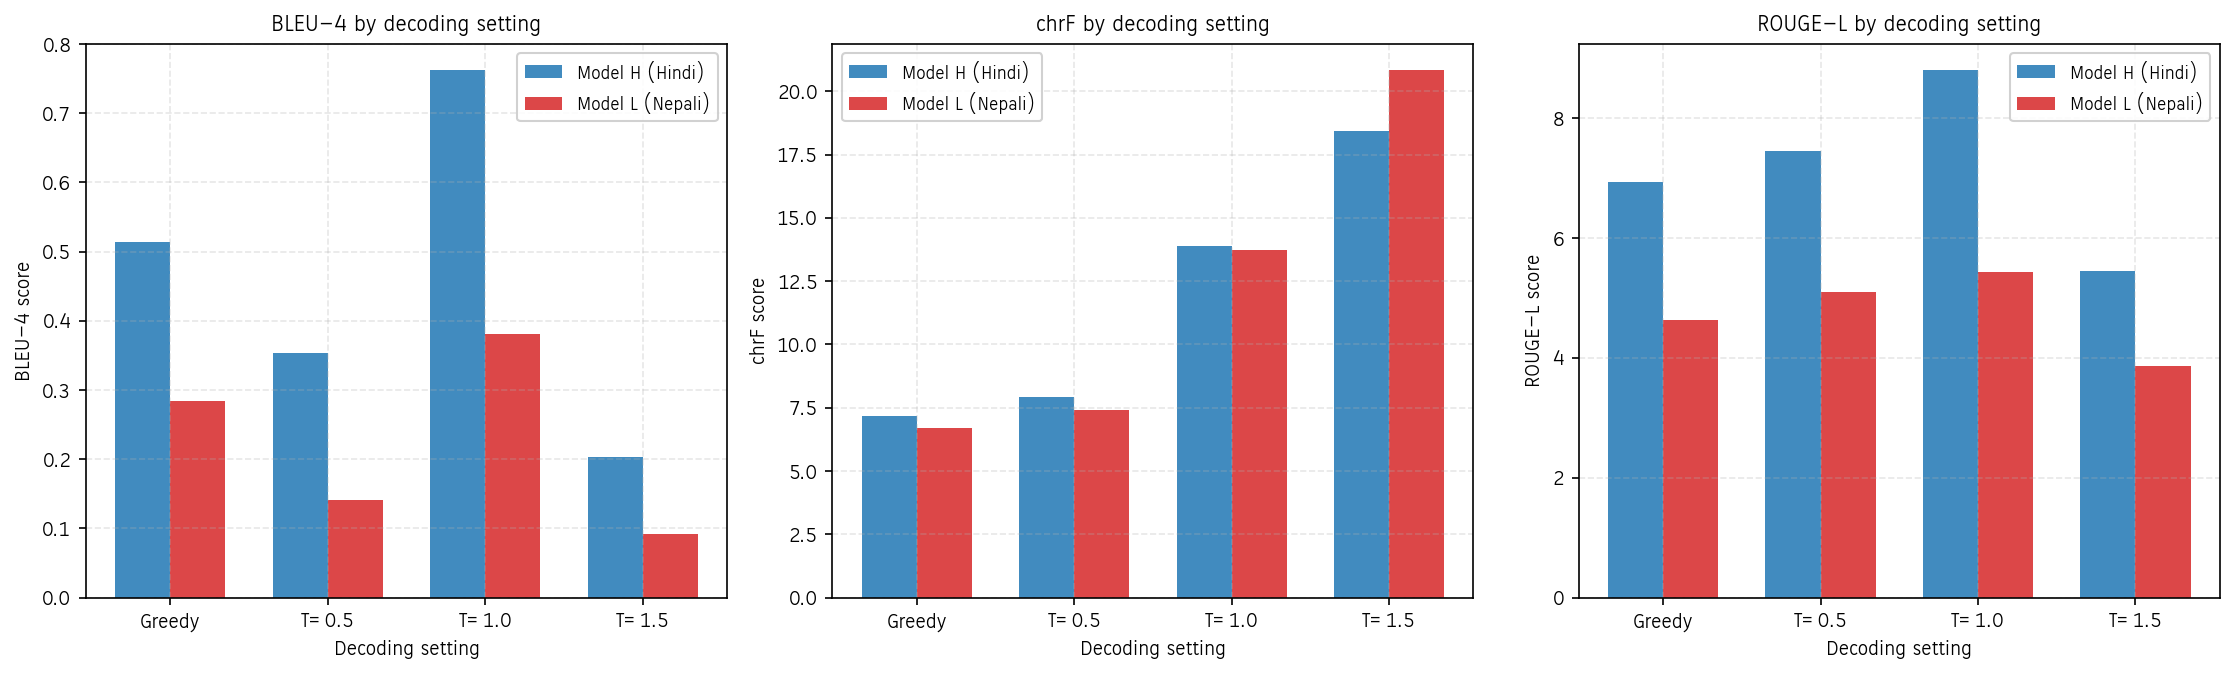
\includegraphics[width=0.48\textwidth]{../figures/comparison/generation_metrics_both.png}
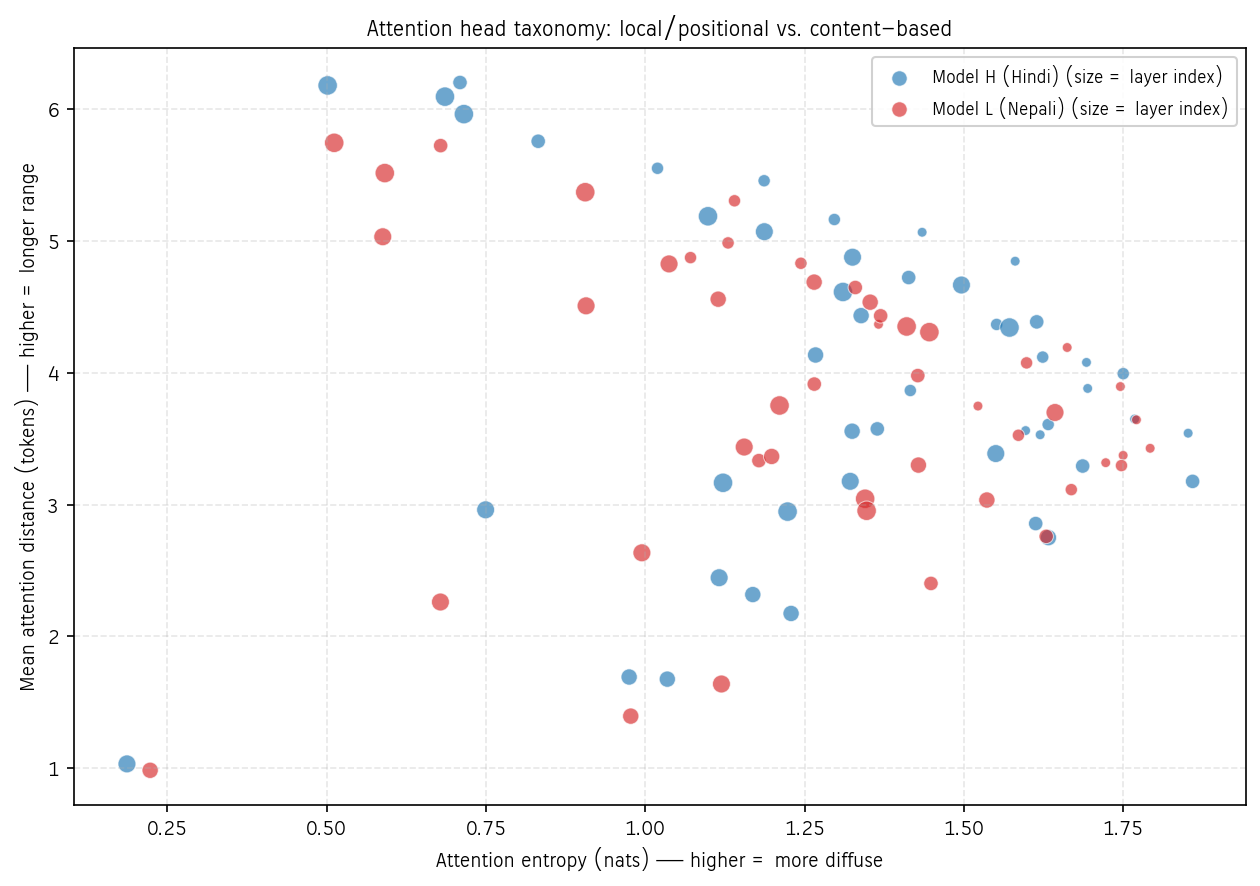
\includegraphics[width=0.48\textwidth]{../figures/comparison/attention_head_taxonomy.png}
\caption{Left: generation-quality metrics (BLEU-4, chrF, ROUGE-L) across decoding settings, both models. Right: local/positional vs.\ content-based head-taxonomy split, both models, 6 layers $\times$ 8 heads each.}
\end{figure}

%=====================================================================
\section{Phase 3 --- Reasoning Finetuning, Attention Analysis}
\label{sec:p3}
%=====================================================================

\textbf{Synthetic reasoning dataset.} Own synthetic dataset per language (not downloaded), four attribute domains (age, height, price, quantity) $\times$ two task types (pairwise; 3-entity transitive chains) $\times$ four paraphrased templates (3 trained on, 1 held out entirely for wording generalization). 2,400 train / 320 each of validation, test\_seen, test\_unseen\_entity, test\_unseen\_wording, per language. \textbf{Leakage control}: each domain's entity pool is split once into disjoint train/test name sets before any example is generated; \texttt{test\_seen} draws only train names, the two unseen splits draw only test names, independently of the held-out-template axis.

\textbf{Finetuning protocol and why this specific recipe.} Each model finetuned independently from its own Phase 2 \texttt{best.pt}, tokenizer/vocabulary fixed (no new tokens added --- an explicit \texttt{<ANS>}-style marker was considered and rejected specifically because it would force resizing the embedding table, breaking the ``tokenizer/vocabulary fixed'' constraint), loss masked to the answer span only via \texttt{ignore\_index=-100} (the model still attends to the full prompt in its forward pass; only the backward pass ignores prompt-token loss). Full finetuning rather than LoRA/PEFT: at 24.4M parameters the whole model finetunes in under 2 minutes per epoch on modest hardware, well inside the budget where PEFT's memory-saving motivation (relevant at 7B+ scale) actually applies --- adding PEFT machinery here would be complexity without a corresponding benefit. Identical recipe deliberately used for \emph{both} languages: LR $10^{-4}\to10^{-5}$ (cosine, 5\% warmup), 4 epochs, batch 16, AdamW (0.9, 0.95), seed 42, 600 total steps ($\sim$12 min Hindi / $\sim$25 min Nepali wall-clock, CPU) --- so that any Model H vs.\ Model L gap in the results below is attributable to data/language, not to a finetuning-recipe difference, mirroring the same identical-hyperparameter discipline used for the Phase 2 architecture.

\textbf{This recipe is a diagnosed fix, not a first guess.} A first-round run (24-name entity pool, 6 epochs, higher LR) scored 0.422 on \texttt{test\_seen} but exactly \textbf{0.000} on both unseen splits --- the course's own memorization case study reproduced almost exactly: at only 24 names across 2,400 training examples, each name appears $\sim$100 times, cheap enough to memorize name$\to$answer mappings instead of learning the comparison itself. The fix applied two independent levers rather than one, so the cause of any improvement would be traceable: (i) entity pools enlarged 24$\to$80 names (cutting per-name repetition to $\sim$30, a $\sim$3$\times$ reduction), and (ii) epochs lowered 6$\to$4 and peak LR lowered to the $10^{-4}$ floor the course SFT guidance gives, watched via a per-epoch unseen-entity accuracy probe logged during training rather than only checked after the fact. The numbers reported below are from this corrected, retrained run.

\begin{table}[h]
\centering\small
\begin{tabular}{llrrr}
\toprule
\textbf{Test split} & \textbf{Model} & \textbf{Pretrained} & \textbf{Finetuned} & \textbf{$\Delta$} \\
\midrule
Seen entity + seen wording & H (Hindi) & 0.000 & 0.412 & +0.412 \\
Unseen entity + seen wording & H (Hindi) & 0.000 & 0.066 & +0.066 \\
Unseen entity + unseen wording & H (Hindi) & 0.000 & 0.059 & +0.059 \\
Seen entity + seen wording & L (Nepali) & 0.000 & 0.434 & +0.434 \\
Unseen entity + seen wording & L (Nepali) & 0.000 & 0.191 & +0.191 \\
Unseen entity + unseen wording & L (Nepali) & 0.000 & 0.203 & +0.203 \\
\bottomrule
\end{tabular}
\caption{Three-way reasoning exact-match accuracy, pretrained-only vs.\ finetuned (mean over 3 seeds; greedy decoding, so seeds are a correctness check, not a variance estimate).}
\end{table}

\textbf{Notable reversal.} Model L (Nepali) generalizes \emph{more} reliably than Model H (Hindi) on both held-out axes (unseen-entity 0.191 vs.\ 0.066; unseen-wording 0.203 vs.\ 0.059), despite being the lower-resource model throughout Phases 1--2. This is the opposite direction from every raw token-level Phase 1--2 metric. Per the SFT format-vs-substance distinction, this is read as a difference in what each pretrained base could already do latently, not as evidence Nepali's language modelling is stronger (Phase 2 showed the opposite on perplexity, and BPB showed the two nearly tied).

\begin{table}[h]
\centering\small
\begin{tabular}{lrr}
\toprule
& \textbf{Before SFT} & \textbf{After SFT} \\
\midrule
Model H pretraining-val PPL & 26.38 & 38.55 \\
Model L pretraining-val PPL & 42.32 & 65.47 \\
\bottomrule
\end{tabular}
\caption{Catastrophic-forgetting diagnostic: PPL on the \emph{original} Phase 2 pretraining validation set, before/after reasoning SFT. Expected to rise (narrow synthetic distribution); this measures distribution shift, not reasoning success.}
\end{table}

\textbf{Error provenance (quantified, not just illustrated).} Every wrong prediction on both unseen splits was classified programmatically against each language's own train/test entity pools:

\begin{table}[h]
\centering\footnotesize
\begin{tabular}{llrrrrr}
\toprule
\textbf{Lang.} & \textbf{Task} & \textbf{n wrong} & \textbf{Train-pool halluc.} & \textbf{Malformed} & \textbf{Legal wrong entity} & \textbf{Empty/other} \\
\midrule
H & pairwise & 291 & 77.3\% & 9.3\% & 9.3\% & 4.1\% \\
H & transitive3 & 309 & 85.4\% & 3.6\% & 4.9\% & 6.1\% \\
L & pairwise & 240 & 58.8\% & 8.3\% & 25.4\% & 7.5\% \\
L & transitive3 & 274 & 47.4\% & 2.2\% & 44.9\% & 5.5\% \\
\bottomrule
\end{tabular}
\caption{Error-provenance classification (\texttt{shared/eval/error\_provenance.py}). Hindi's errors are dominated by hallucinating a training-pool name (memorization); Nepali more often names the \emph{other} real entity in the prompt (\emph{legal but wrong entity}, 25--45\%) rather than hallucinating --- a genuinely different, more prompt-engaged failure mode, consistent with Nepali's stronger unseen-split accuracy above.}
\end{table}

\begin{figure}[h]
\centering
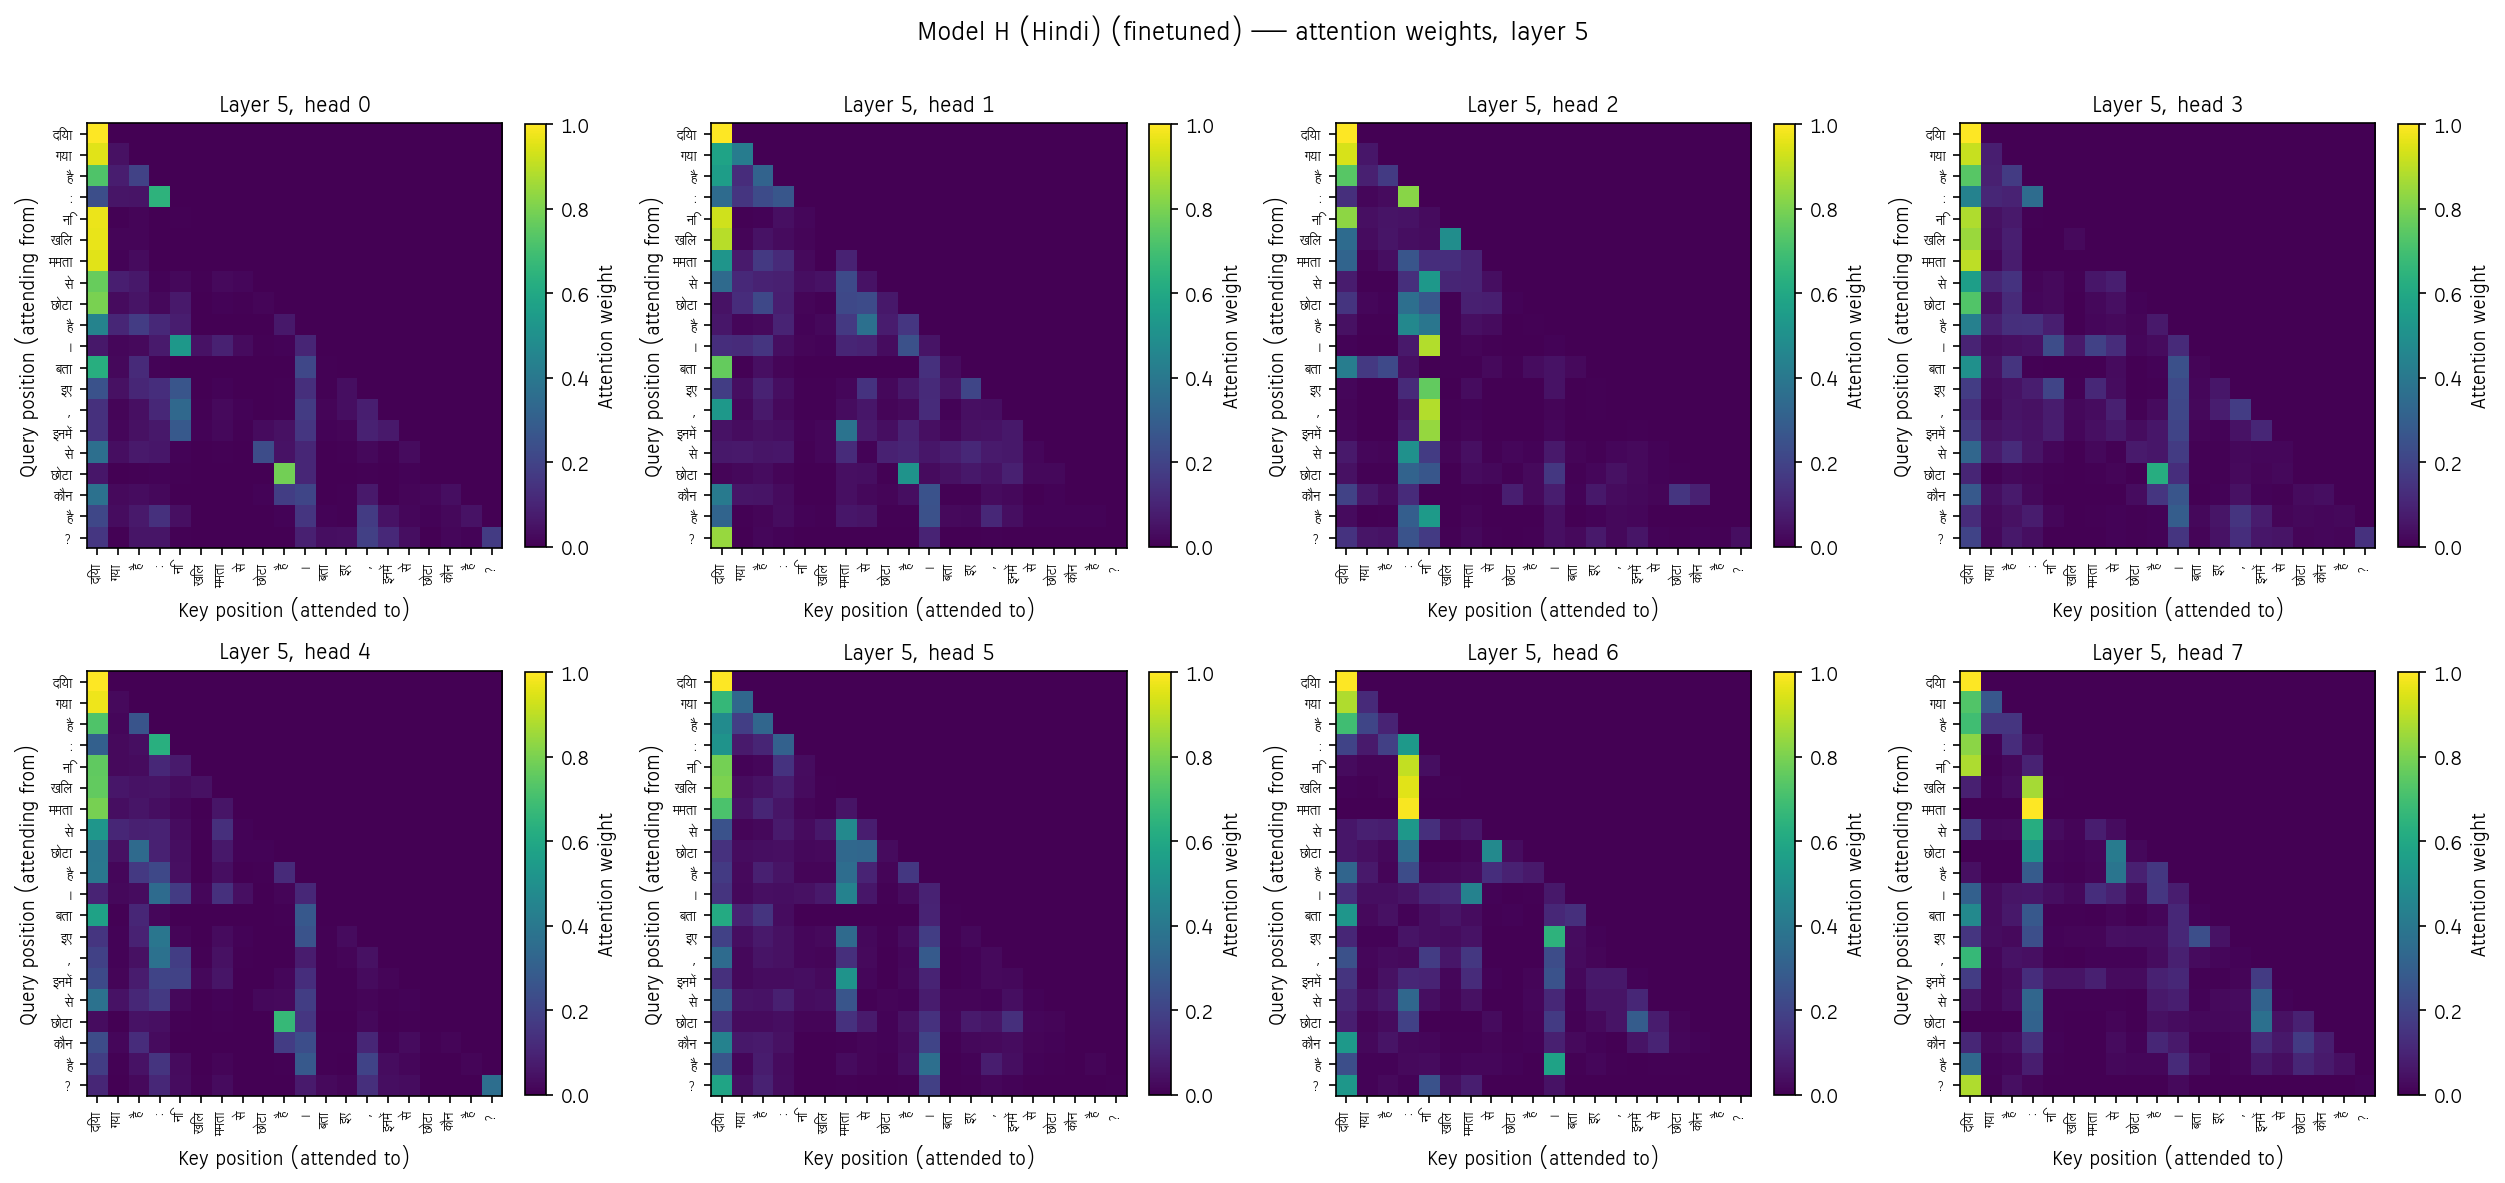
\includegraphics[width=0.31\textwidth]{../figures/hindi/attention_heatmap_hin_finetuned_L5.png}
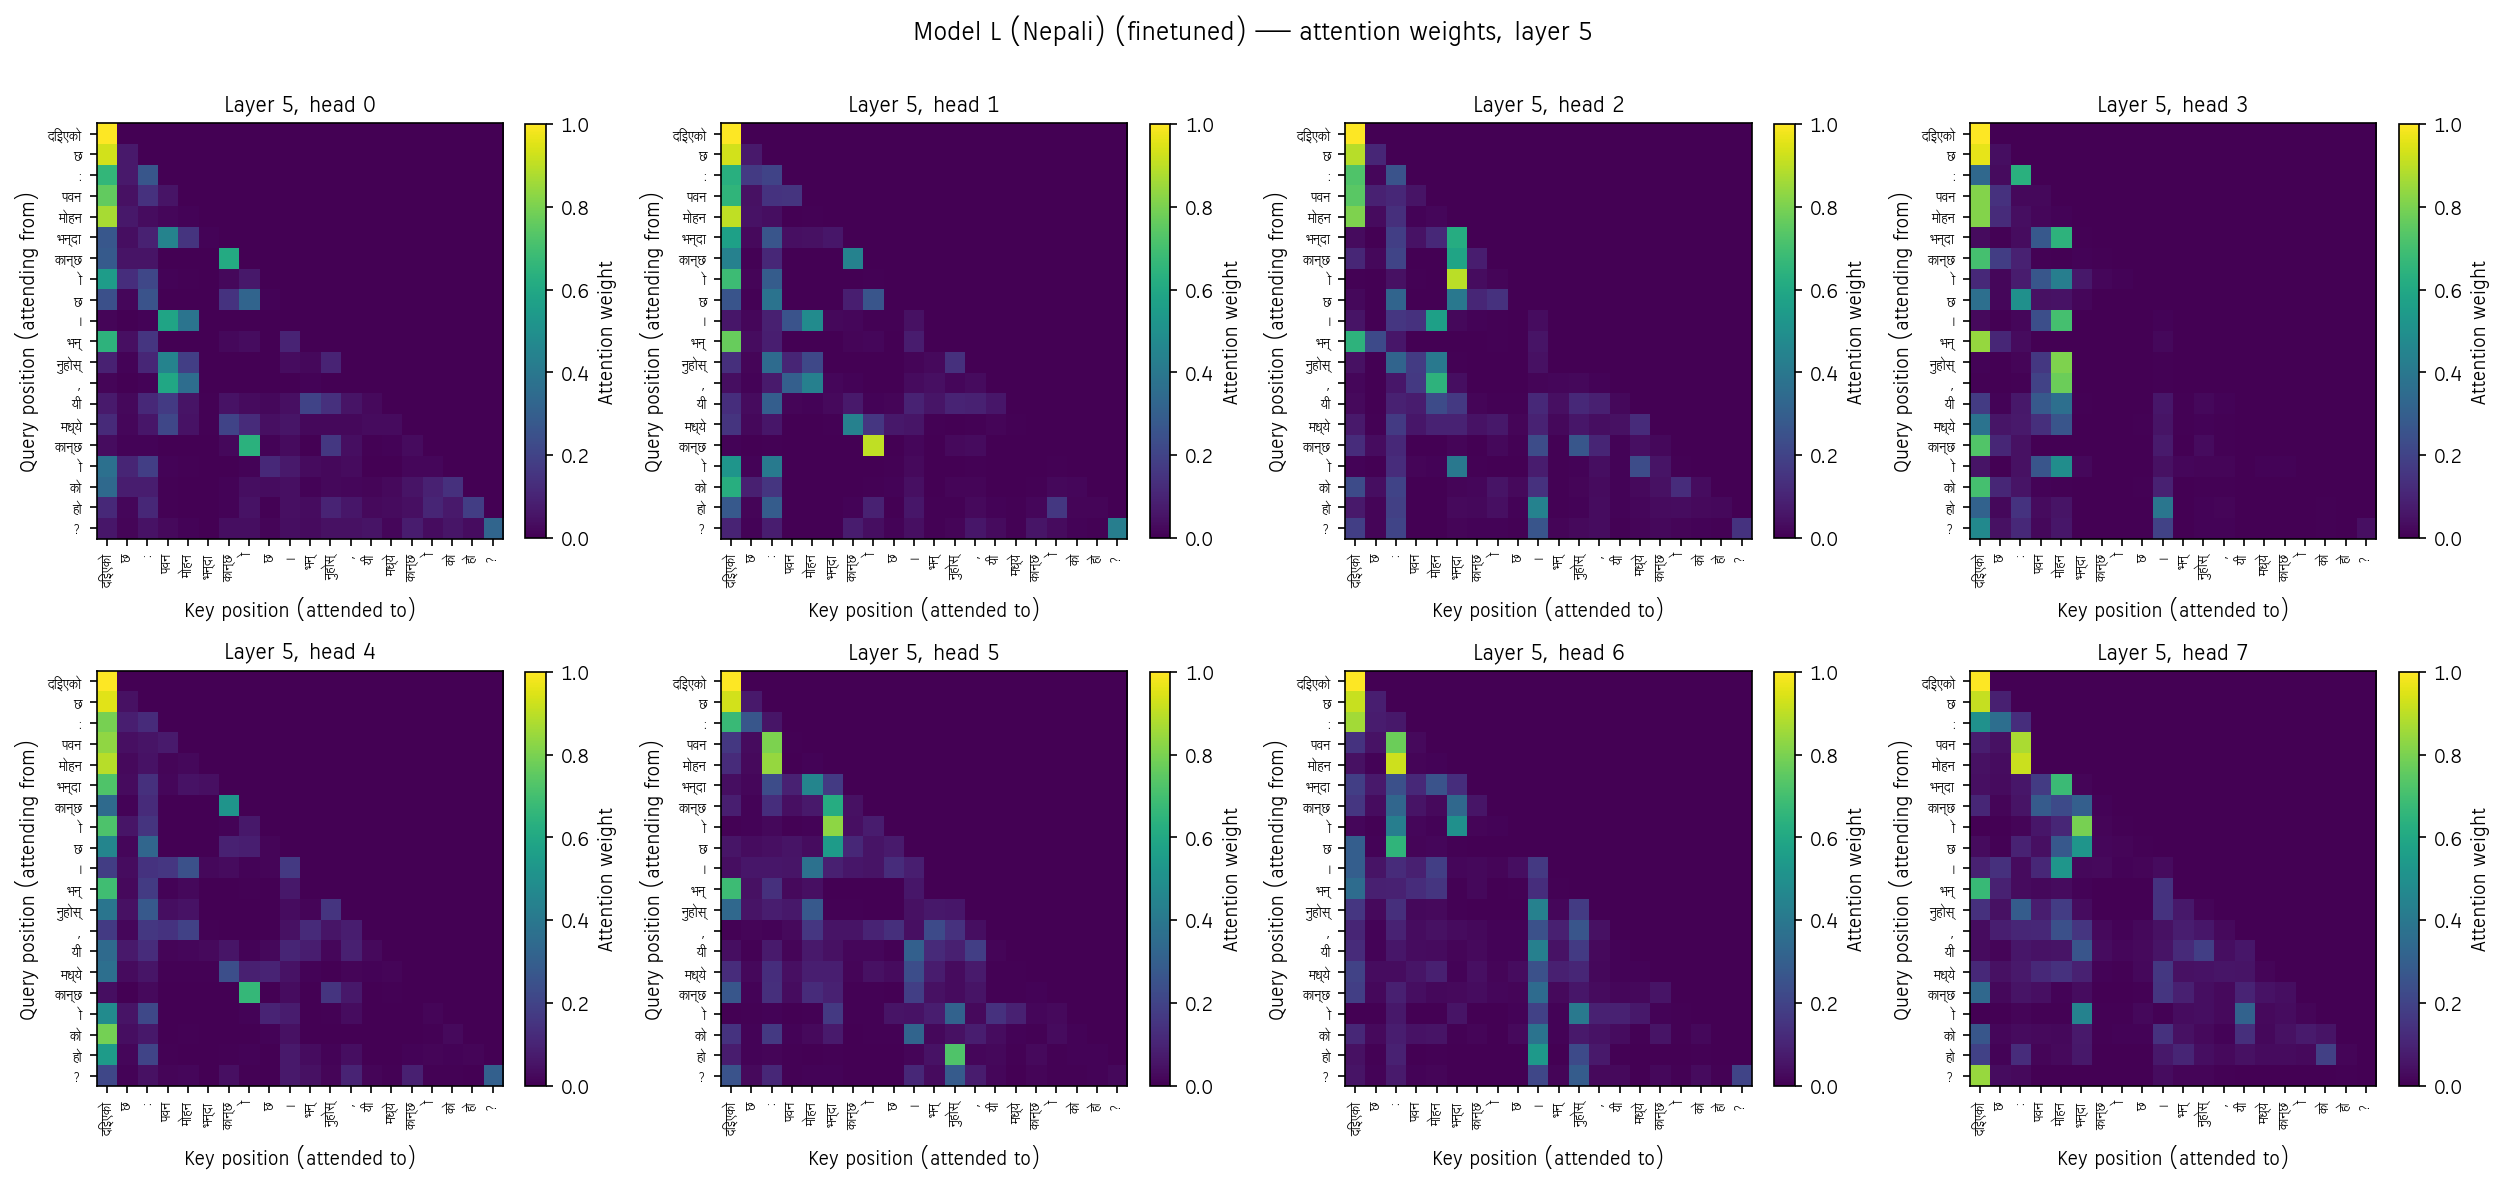
\includegraphics[width=0.31\textwidth]{../figures/nepali/attention_heatmap_nep_finetuned_L5.png}
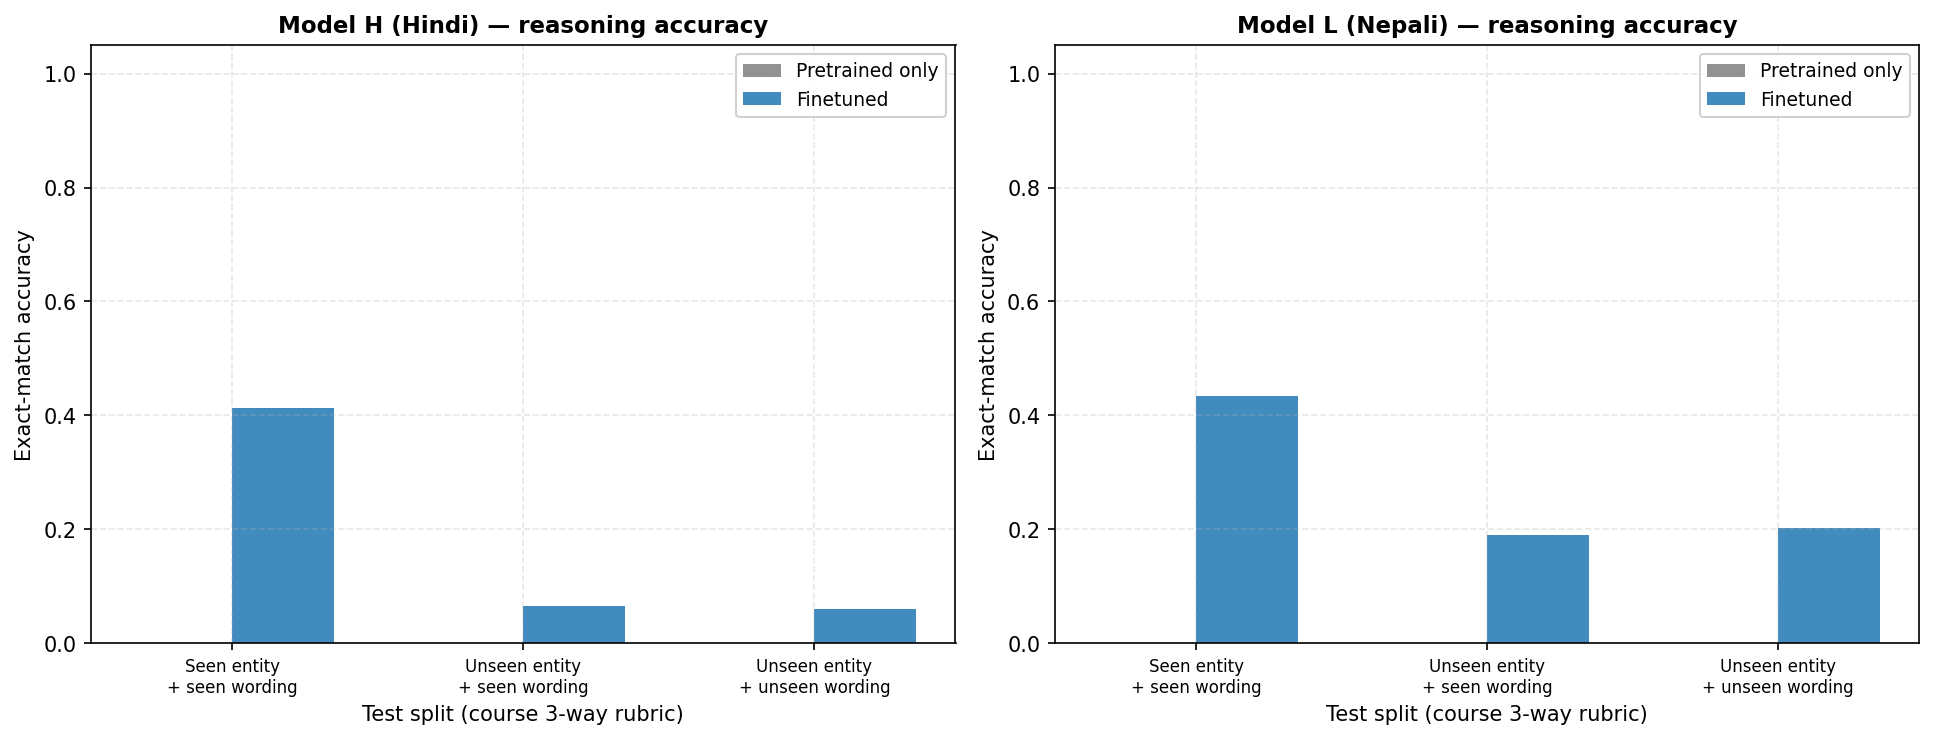
\includegraphics[width=0.31\textwidth]{../figures/comparison/reasoning_accuracy_3way.png}
\caption{Left/middle: late-layer (L5) post-finetune attention heatmaps, Hindi and Nepali, on the same comparative-reasoning prompt structure --- the pretrained global first-token sink is replaced by a content-specific anchor in both languages after finetuning. Right: three-way accuracy comparison, both models.}
\end{figure}

Finetuning \textbf{sharpens} late-layer attention (mean entropy: H $1.5936\to1.5585$, L $1.6193\to1.6163$) while lengthening mean attention distance slightly (H $4.86\to5.02$, L $4.95\to5.08$ tokens) --- consistent with heads reorganizing toward a fixed content anchor rather than a purely positional pattern, in both languages independently.

%=====================================================================
\section{Cross-Phase Metrics Comparison}
%=====================================================================

Every major H-vs-L metric from all three phases, side by side, with which model ``wins'' and by what margin --- the single table that makes \S\ref{sec:final-comparison}'s answer to Question 2 checkable at a glance.

\begin{table}[h]
\centering\footnotesize
\begin{tabular}{lp{2.6cm}rrl}
\toprule
\textbf{Phase} & \textbf{Metric} & \textbf{Model H} & \textbf{Model L} & \textbf{Favors / gap} \\
\midrule
1 & Train tokens & 632.4M & 637.5M & tied ($<$1\% apart) \\
1 & Manual-lane share & 18.1\% & 18.3\% & tied \\
1 & Unique whitespace words & 3.96M & 6.80M & L has 1.7$\times$ more (morphology) \\
1 & Tokenizer fertility (tok/word) & \textbf{1.3042} & 1.4394 & \textbf{H} by 10.4\% (fewer tokens/word) \\
2 & Validation perplexity & \textbf{26.21} & 41.52 & \textbf{H} by 58.4\% (token space) \\
2 & Validation BPB (byte space) & 0.4797 & \textbf{0.4635} & \textbf{L} by 3.4\% (tokenizer-fair) \\
2 & Mean attention entropy & 1.3109 & 1.2671 & L sharper (more local) \\
2 & Generation chrF range (greedy$\to$T1.5) & 7.16--18.44 & 6.71--20.84 & L wider spread at high T \\
2 & Greedy repetition rate & \textbf{0.70} & 0.76 & \textbf{H} slightly less repetitive \\
3 & Reasoning acc., seen/seen & 0.412 & \textbf{0.434} & \textbf{L} by 0.022 \\
3 & Reasoning acc., unseen entity & 0.066 & \textbf{0.191} & \textbf{L} by 0.125 (2.9$\times$) \\
3 & Reasoning acc., unseen wording & 0.059 & \textbf{0.203} & \textbf{L} by 0.144 (3.4$\times$) \\
3 & Forgetting: PPL rise factor after SFT & 1.46$\times$ & 1.55$\times$ & H forgets slightly less \\
3 & Error type: train-pool hallucination & 77--85\% & 47--59\% & H memorizes more \\
\bottomrule
\end{tabular}
\caption{All H-vs-L metrics across the project, one table. \textbf{Bold} marks the higher-resource-favoring or lower-resource-favoring value per row where a clear winner exists. Note the pattern: every Phase 1 raw-scale metric is tied, every Phase 2 \emph{token-space} metric favors H, but BPB (byte-space, tokenizer-fair) and all three Phase 3 reasoning-generalization metrics favor L --- the resource-tier story is not monotonic across metrics.}
\label{tab:crossphase}
\end{table}

%=====================================================================
\section{Final Comparison --- the Four Required Questions}
\label{sec:final-comparison}
%=====================================================================

\textbf{1. How did data scale and quality differ between Model H and Model L?}
Scale is near-identical (648.0M vs.\ 659.5M train tokens; both exceed the 500M target by 26--28\%, both clear the $\geq$20\% manual floor) --- \emph{not} the differentiator. The real asymmetry is morphological: Nepali's agglutinative case-marking produces 6.80M unique surface forms against Hindi's 3.96M at comparable corpus size, and 10.4\% higher tokenizer fertility (1.4394 vs.\ 1.3042).

\textbf{2. How do language-modeling and reasoning results compare across the two resource tiers?}
Phase 2: Model L is 58.4\% worse on perplexity but 3.4\% \emph{better} on BPB --- the token-space gap is a tokenizer artifact. Phase 3 reasoning accuracy is the first metric in this project measuring genuinely learned behavior rather than distributional fit, and it does \emph{not} favor Model H either: Model L reaches 0.191/0.203 on unseen-entity/unseen-wording against Model H's 0.066/0.059. Across the full cross-phase comparison (Table~\ref{tab:crossphase}), only token-space perplexity clearly favors the higher-resource model --- every scale metric is tied, and BPB plus all three reasoning-generalization metrics favor the lower-resource model.

\textbf{3. What tokenizer/corpus factors most affected the lower-resource model?}
Fertility is the dominant, well-evidenced factor for Phase 1--2 results (BPB reversal). It does \emph{not}, however, explain the Phase 3 \texttt{transitive3} Hindi-vs-Nepali gap on the higher-resource model's own error profile: the one concrete tokenizer-level hypothesis tested for that gap (inconsistent subword segmentation of Nepali's glued comparative \dn{भन्दा}) was checked directly against the tokenizer and refuted. This is reported as an open question, not force-fit to the fertility story that explains the unrelated Phase 2 result.

\textbf{4. What evidence explains the observed differences?}
Direct inspection of per-example predictions (not aggregate accuracy alone) is what actually explains the failure modes: Hindi's wrong answers are dominated by clean hallucinations of familiar training-pool names (77--85\%), evidence of entity-identity memorization rather than genuine comparison; Nepali more often names the \emph{other} real entity in the prompt (25--45\% ``legal but wrong entity''), evidence it is at least reading the prompt's own entities even when it errs. The attention comparison adds a mechanistic layer: finetuning sharpens late-layer attention onto content-specific positions (replacing the pretrained attention sink) in both languages independently, which is direct evidence of \emph{where} each model's internal computation changed, not just that its outputs did.

%=====================================================================
\section{Where Automation Substitutes for Human Judgment}
%=====================================================================
\begin{itemize}
\item \textbf{No fluent reader assessed retained/rejected corpus text (Phase 1).} Script-filter ratios, quality heuristics, and the 0.4 near-duplicate similarity threshold are conventional/algorithmic choices, not tuned against sampled Hindi/Nepali text.
\item \textbf{Generation quality (Phase 2) was scored by metrics, not a fluent reader}; qualitative examples are shown as evidence of grammaticality only.
\item \textbf{Attention head labels (Phases 2--3) are statistical} (median-split on entropy/distance), not interpretively verified against what a head actually attends to linguistically.
\item \textbf{Reasoning template naturalness (Phase 3)} was reviewed by a fluent speaker for the 12 distinct sentence patterns per language (not all $\sim$6,000 rendered examples individually), and one real Nepali compounding bug was found and fixed before the final finetuning run reported above.
\item \textbf{The Hindi/Nepali \texttt{transitive3} generalization gap} is reported with one tested-and-refuted tokenizer hypothesis and no confirmed replacement cause --- an honest open question, not a manufactured explanation.
\end{itemize}

%=====================================================================
\section{Reproduction}
%=====================================================================
\begin{footnotesize}
\begin{verbatim}
# Phase 1 (per language; replace hindi -> nepali for Model L)
python hindi/scripts/01_download_indiccorp.py  ...  python hindi/scripts/12_tokenize_corpus.py
  # (stages 01-12 in order; see hindi/Hindi_Corpus_Pipeline_Run_Instructions.md)
# Phase 2
python hindi/train/pretrain.py                       # resumes automatically from checkpoint
python hindi/eval/evaluate_lm.py --checkpoint hindi/checkpoints/best.pt
python hindi/eval/evaluate_generation.py --checkpoint hindi/checkpoints/best.pt
python hindi/eval/analyze_attention.py --checkpoint hindi/checkpoints/best.pt
# Phase 3
python hindi/reasoning_data/generate_dataset.py
python hindi/finetune/finetune.py                     # resumes automatically
python hindi/eval/evaluate_reasoning.py --device cpu  # 3-way accuracy + PPL before/after
python hindi/eval/compare_attention.py --device cpu
python report/scripts/make_phase2_figures.py && python report/scripts/make_phase3_figures.py
python report/scripts/build_phase2_report.py && python report/scripts/build_phase3_report.py
python -m pytest tests/test_phase2.py tests/test_phase3.py -v   # 22 + 23 correctness gates
\end{verbatim}
\end{footnotesize}
Full per-phase step-by-step instructions, exact config keys, and all Google Drive links (raw/final corpora, pretrained checkpoints, finetuned checkpoints, both languages) are in the top-level \texttt{README.md}. Per-phase detail, all figures, and complete tables live in \texttt{report/phase1\_report.md}, \texttt{phase2\_report.md}, \texttt{phase3\_report.md}.

\end{document}
